\documentclass[aspectratio=169]{beamer}
\usetheme{hogent}
\usecolortheme{hgwhite} % witte achtergrond, zwarte tekst

%% common.tex -- Code die in elk .tex-bestand terug komt

%% Packages

\usepackage[dutch]{babel}
\usepackage{graphicx}
\usepackage{comment,enumerate,hyperref}
\usepackage{amsmath,amsfonts,amssymb}
\usepackage{eurosym}
\usepackage{booktabs}
\usepackage{multicol,multirow}
\usepackage{listings}

\usepackage[outputdir=out]{minted}
%\usepackage{minted}

\usepackage[backend=biber,style=apa]{biblatex}
\DeclareLanguageMapping{dutch}{dutch-apa}

\usepackage{csquotes}

%% Variabelen, elk academiejaar aan te passen
\newcommand{\academicyear}{2023--2024 (revisie: \today)}
\newcommand{\lecturers}{Thomas Aelbrecht \and Thomas Parmentier \and Bert Van Vreckem}
\newcommand{\coursename}{Research Methods (IT)}

%% Macro's en commando's

%% \alertbox: een kader voor tekst die moet opvallen
\newcommand{\alertbox}[2][hgblue]{%
  \setbeamercolor{alertbox}{bg=#1,fg=white}
  \begin{beamercolorbox}[sep=2pt,center]{alertbox}
    \textbf{#2}
  \end{beamercolorbox}
}


\addbibresource{rm4-bibliografie.bib}

%---------- Info over de presentatie ------------------------------------------

\title{Module 2. Werken met \LaTeX.}
\subtitle{\coursename}
\author{\lecturers}   % Pas waarden aan in common.tex
\date{\academicyear}

\begin{document}

\begin{frame}
  \maketitle
\end{frame}

\begin{frame}
  \frametitle{Inhoud}

  \tableofcontents
\end{frame}

\section{Inleiding}

\subsection{Filosofie, geschiedenis}

\begin{frame}
  \frametitle{Filosofie: waarom {\LaTeX}?}

  \begin{itemize}
    \item<+-> WYSIWYG tekstverwerkers dwingen auteurs om de vormgeving te verzorgen.
    \item<+-> Gevolg is slechte, inconsistente opmaak van documenten.
    \item<+-> Goede vormgeving van teksten is een \textit{specialisatie}, en wordt best
    uit handen van auteurs genomen.
    \item<+-> {\LaTeX} zorgt dat auteurs enkel over de \textit{inhoud} en \textit{structuur} van de tekst moet nadenken.
  \end{itemize}
\end{frame}

\begin{frame}[plain]
  \frametitle{Geschiedenis}

  \begin{columns}[c]

    \column{.67\textwidth}
    \begin{itemize}
      \item<+-> 1977: Donald Knuth vindt de drukproeven van zijn boek \textit{The art of Computer Programming} afschuwelijk
      \item<+-> 1978: Schreef dan maar zelf een tekstzetsysteem, {\TeX}
      \item<+-> 1989: Versie 3.0, sindsdien enkel bugfix-releases (convergeren naar \(\pi\))
      \item<+-> 1980s: Leslie Lamport ontwikkelt markup-taal voor {\TeX}: {\LaTeX}
    \end{itemize}

    \column{.33\textwidth}
    \begin{center}
      \only<1-3>{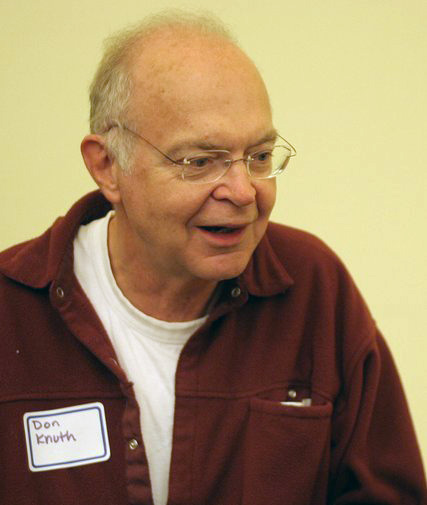
\includegraphics[width=\textwidth]{1/donald-knuth}}
      \only<4->{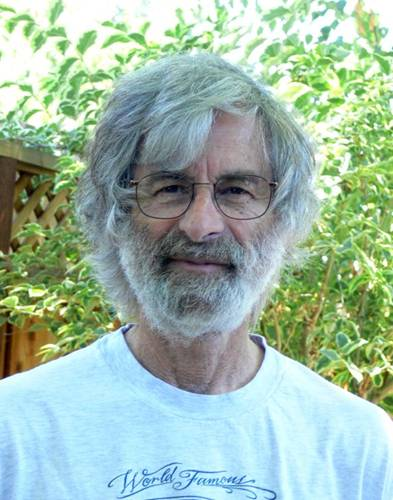
\includegraphics[width=\textwidth]{1/leslie-lamport}}
    \end{center}

  \end{columns}
\end{frame}

\subsection{Voorbeelden}

\begin{frame}
  \frametitle{Voorbeelden---papers}

  {\LaTeX} is de norm voor wetenschappelijke publicaties in computerwetenschappen, wiskunde, fysica, enz.

  \begin{center}
    
\includegraphics[height=.6\textheight]{1/latex-paper}
  \end{center}

\end{frame}

\begin{frame}
  \frametitle{Voorbeelden---boeken}

  Ook: cursussen, thesissen, enz.

  \begin{center}
    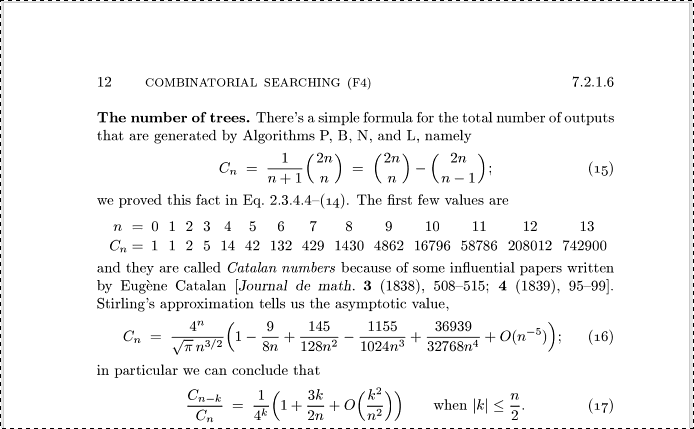
\includegraphics[height=.6\textheight]{1/latex-book}
  \end{center}

\end{frame}

\begin{frame}
  \frametitle{Voorbeelden---presentaties}

  \begin{center}
    vb.\ deze presentatie\ldots
  \end{center}

\end{frame}

\begin{frame}
  \frametitle{Voordelen}

  \begin{itemize}
    \item<+-> Enkel bekommeren om inhoud, goede en consistente opmaak gegarandeerd.
    \item<+-> Stijl aanpassen zonder inhoud te wijzigen.
    \item<+-> Tekstformaat \(\Rightarrow\) geschikt voor versiebeheersysteem!
    \item<+-> Is de norm in verschillende onderzoeksdomeinen, o.a.\ computerwetenschappen
  \end{itemize}
\end{frame}


\begin{frame}
  \frametitle{Nadelen}

  \begin{itemize}
    \item<+-> Zware leercurve \(\Rightarrow\) copy paste voorbeelden, gebruik infobronnen, vraag hulp
    \item<+-> Soms is gewenste opmaak niet eenvoudig te bereiken (vb.~tabellen)
  \end{itemize}

  \uncover<1->{%
    \begin{center}
      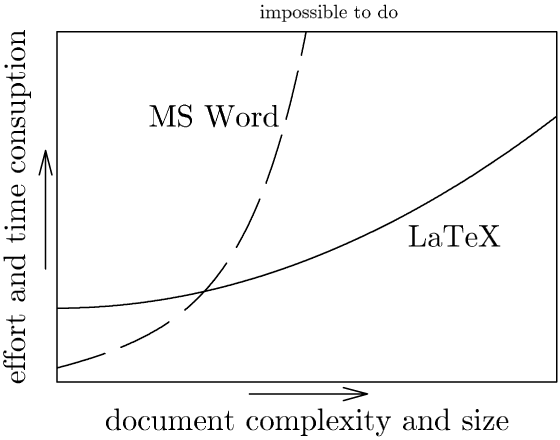
\includegraphics[height=.5\textheight]{1/word-vs-latex}
  \end{center}}
\end{frame}

\subsection{Hulp zoeken}

\begin{frame}
  \frametitle{Hulp zoeken}

  \begin{itemize}
    \item Tobias Oetiker, et al., \emph{The Not So Short Introduction to {\LaTeXe}}, (a.k.a. ``lshort''):
    \url{https://tobi.oetiker.ch/lshort/lshort.pdf}
    \item {\TeX} --- {\LaTeX} StackExchange (Q \& A site): \url{http://tex.stackexchange.com/}
    \item \emph{{\LaTeX} Wikibook}, \url{http://en.wikibooks.org/wiki/LaTeX}
    \item Handleidingen van packages (pdf) via bv. \url{https://ctan.org/pkg/}
  \end{itemize}

\end{frame}

\section{Aan de slag met {\LaTeX}}

\subsection{Documentstructuur}

\begin{frame}
  \frametitle{Werkwijze}

  \begin{itemize}
    \item<+-> Schrijf tekst in {\LaTeX}\\
    = tekstbestand! (markuptaal zoals HTML)
    \item<+-> Compileer (evt.\ verschillende keren)
    \item<+-> Bekijk resultaat in PDF
  \end{itemize}
\end{frame}

\begin{frame}[fragile]
  \frametitle{{\LaTeX} commando's}

  \begin{block}{Basis-syntax}
    \verb|\commandonaam[optionele,argumenten]{arg1}{arg2}|
  \end{block}

  \pause

  Bijvoorbeeld:

  \begin{itemize}
    \item<+-> \verb|\documentclass[a4paper,12pt,twocolumn]{article}|
    \item<+-> \verb|\'{e}l\`{e}ve| \(\Rightarrow\) \'el\`eve
    \item<+-> \verb|\begin{itemize}|\\
    \verb|\item lijst|\\
    \verb|\end{itemize}|
  \end{itemize}

\end{frame}

\begin{frame}[fragile]
  \frametitle{Een document opbouwen}

  \begin{center}
    \alert{%
      \only<1>{Definitie documentsoort (hier: artikel)}
      \only<2>{``body'' van het document}
      \only<3>{Documentinhoud}
      \only<4>{Extra functionaliteit beschikbaar maken}
      \only<5>{Titel, auteur komt in ``preamble''}
      \only<6>{Titel in document invoegen}
    }
  \end{center}

  \begin{semiverbatim}
    \uncover<1->{\alert<1>{\\documentclass[a4paper,12pt]\{article\}}}
    \uncover<4->{\alert<4>{\\usepackage[dutch]\{babel\}}}
    \uncover<5->{\alert<5>{\\title\{Minimaal \{\\LaTeX\} document\}}}
    \uncover<5->{\alert<5>{\\author\{Bert \{Van Vreckem\}\}}}
    \uncover<5->{\alert<5>{\\date\{\\today\}}}
    \uncover<2->{\alert<2>{\\begin\{document\}}}
    \uncover<6->{\alert<6>{\\maketitle}}
    \uncover<3->{\alert<3>{Lorem ipsum dolor sit amet, consectetur adipiscing elit.}}
    \uncover<2->{\alert<2>{\\end\{document\}}}
  \end{semiverbatim}

\end{frame}

\begin{frame}
  \frametitle{Resultaat}

  \begin{center}
    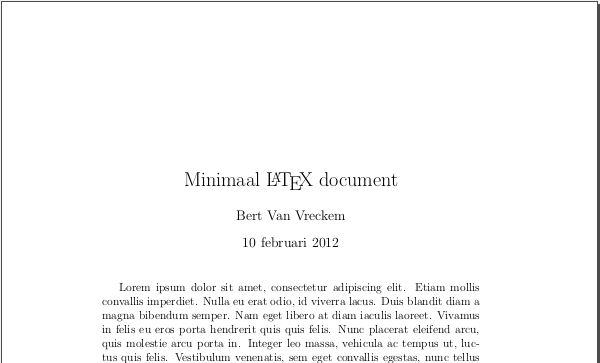
\includegraphics[height=.6\textheight]{1/minimaal-document}
  \end{center}
\end{frame}

\begin{frame}[fragile]
  \frametitle{Documenttypes}

  \begin{center}
    \begin{semiverbatim}
      \\documentclass[\alert<2>{OPTIONS}]\{\alert<1>{TYPE}\}
    \end{semiverbatim}
  \end{center}

  \only<1>{%
    \begin{center}
      \begin{tabular}{ll}
        \toprule
        TYPE & soort document \\
        \midrule
        \texttt{article} & artikel, paper, korte tekst \\
        \texttt{beamer} & presentatie \\
        \texttt{book} & boek \\
        \texttt{report} & (lang) rapport, thesis, verslag, \ldots \\
      \end{tabular}
    \end{center}
  }
  \only<2>{%
    \begin{center}
      \begin{tabular}{ll}
        \toprule
        OPTION & soort document \\
        \midrule
        \texttt{12pt} & 12-puntsletters (ipv 10pt) \\
        \texttt{a4paper} & A4 (ipv Am. Letter) \\
        \texttt{twocolumn} & gebruikelijk bij artikels \\
        \texttt{twoside} & voor dubbelzijdig afdrukken \\
      \end{tabular}
    \end{center}
  }
\end{frame}

\begin{frame}[fragile]
  \frametitle{Documentstructuur}

  \begin{center}
    \begin{tabular}{ll}
      \verb?\part? & (geen invloed op hoofdstuknummers) \\
      \verb?\chapter? & (enkel in \texttt{book}, \texttt{report}) \\
      \verb?\section? & \\
      \verb?\subsection? & \\
      \verb?\subsubsection? & (niet in \texttt{book}, \texttt{report}) \\
      \verb?\paragraph? & \\
      \verb?\subparagraph? & \\
      &\\
      \verb?\appendix? & vanaf hier wordt \verb?\chapter? een Bijlage \\
      \verb?\label{?\texttt{\ldots}\verb?}? & voor verwijzingen (met \verb|\ref{LABEL}|)
    \end{tabular}
  \end{center}
\end{frame}

\begin{frame}[fragile]
  \frametitle{Preamble---Nuttige packages}

  \begin{description}
    \item[\texttt{\textbackslash{}usepackage\{amsfonts\}}] AMS math packages: extra wiskundige
    \item[\texttt{\textbackslash{}usepackage\{amsmath\}}] symbolen (o.a.\ getallenverzamelingen
    \item[\texttt{\textbackslash{}usepackage\{amssymb\}}] \(\mathbb{N}, \mathbb{R}, \mathbb{Z}, \mathbb{Q}\), etc.)
    \pause
    \item[\texttt{\textbackslash{}usepackage[dutch]\{babel\}}] Taalinstellingen: woordsplitsingen, commando's voor speciale karakters (``dutch'' voor NL)
    \pause
    \item[\texttt{\textbackslash{}usepackage\{eurosym\}}] Euro-symbool (\euro)
    \pause
    \item[\texttt{\textbackslash{}usepackage\{fancyhdr\}}] Pagina-opmaak met hoofd- en voettekst
    \pause
    \item[\texttt{\textbackslash{}usepackage\{graphicx\}}] Invoegen van figuren \pause
    \item[\texttt{\textbackslash{}usepackage\{lipsum\}}] Vultekst (lorem ipsum dolor sit amet\ldots)
  \end{description}
\end{frame}

\begin{frame}[fragile]
  \frametitle{Preamble---Nuttige packages}

  \begin{description}
    \item[\texttt{\textbackslash{}usepackage[pdftex,bookmarks=true]\{hyperref\}}] PDF krijgt klikbare links \& verwijzingen, inhoudstafel \pause
    \item[\texttt{\textbackslash{}usepackage[utf8]\{inputenc\}}] Accenten gebruiken in tekst (vb. é ipv \verb|\'e|) \pause
    \item[\texttt{\textbackslash{}usepackage\{listings\}}] Broncode mooi opmaken \pause
    \item[\texttt{\textbackslash{}usepackage\{minted\}}] Idem maar vereist Python en Pygments \pause
    \item[\texttt{\textbackslash{}usepackage\{multirow\}}] Tekst over verschillende cellen in tabellen \pause
    \item[\texttt{\textbackslash{}usepackage\{rotating\}}] Tabellen en figuren roteren
  \end{description}
\end{frame}

\subsection{Tekst schrijven}

\begin{frame}[fragile]
 \frametitle{Tekstopmaak}

 \begin{itemize}
    \item<+-> Speciale tekens ({\LaTeX} syntax): \% \$ \& \{ \} \textbackslash{} enz: \\
    \begin{semiverbatim}
      \\\% \\\$ \\\& \\\{ \\\} \\textbackslash\{\}
    \end{semiverbatim}
    \item<+-> Ligaturen: \textrm{fi fl ffi ffl} (automatisch opgemaakt)
    \begin{itemize}
      \item HOGENT font (Montserrat) heeft geen ligaturen
    \end{itemize}
    \item<+-> Accenten: \'{e} \`{e} \^{e} \"{e} \={e} \c{c} enz.
    \begin{semiverbatim}
      \\'\{e\} \\`\{e\} \\^\{e\} \\"\{e\} \\=\{e\} \\c\{c\} enz.
    \end{semiverbatim}
    \item<+-> Ellipsis (\ldots): \texttt{\textbackslash{}ldots}
    \item<+-> Aanhalingstekens: `enkel' ``dubbel''
    \begin{verbatim}
    `enkel' ``dubbel''
    \end{verbatim}
  \end{itemize}
\end{frame}

\begin{frame}[fragile]
 \frametitle{Letterstijlen}

 \begin{center}
   \begin{tabular}{ll}
     \toprule
     Commando & resultaat \\
     \midrule
     \verb?\emph{xxx}?   & \emph{Benadrukken} (\textrm{\emph{cursief}} of \textsf{\emph{`slanted'}})\\
     \verb?\textit{xxx}? & \textit{Cursieve tekst} \\
     \verb?\textbf{xxx}? & \textbf{Vetgedrukte tekst} \\
     \verb?\texttt{xxx}? & \texttt{Monogespatieerde letters} \\
     \verb?\textrm{xxx}? & \textrm{Schreefletters}  \\
     \verb?\textsf{xxx}? & \textsf{Schreefloze letters}  \\
     \verb?\textsc{xxx}? & \textsc{Small Caps} \\
   \end{tabular}
 \end{center}

\end{frame}

\begin{frame}[fragile]
 \frametitle{Lijstomgevingen}

 \begin{columns}[c]
   \column{.49\textwidth}
   \begin{verbatim}
   \begin{itemize}
   \item Een onderdeel
   \item Nog een onderdeel
   \end{itemize}
   \end{verbatim}

   \column{.49\textwidth}
   \begin{itemize}
     \item Een onderdeel
     \item Nog een onderdeel
   \end{itemize}
 \end{columns}

 \pause

 \begin{columns}[c]
   \column{.49\textwidth}
   \begin{verbatim}
   \begin{enumerate}
   \item Een onderdeel
     \begin{enumerate}
     \item extra niveau
     \end{enumerate}
   \item Nog een onderdeel
   \end{enumerate}
   \end{verbatim}

   \column{.49\textwidth}
   \begin{enumerate}
     \item Een onderdeel
     \begin{enumerate}
       \item extra niveau
     \end{enumerate}
     \item Nog een onderdeel
   \end{enumerate}
 \end{columns}

\end{frame}

\subsection{Literatuurlijst}

\begin{frame}[fragile]
  \frametitle{Literatuurlijst}

  \begin{itemize}
    \item<+-> Literatuurlijst is belangrijk onderdeel van een eindwerk
    \item<+-> Strakke regels voor opmaak (HOGENT: APA-stijl)
    \item<+-> {\LaTeX}, meer bepaald Bib{\LaTeX} helpt:
    \begin{itemize}
      \item<+-> ``bibliografische databank'' (in tekstformaat)
      \item<+-> Automatisch correcte opmaak
      \item<+-> Verwijzingen vanuit uit de tekst (\verb|\textcite{}|)
      \item<+-> Ondersteuning via externe tools (bv. JabRef, Mendeley Desktop)
    \end{itemize}
  \end{itemize}

  \pause Zie vervolg cursus!
\end{frame}

\section{Tot slot}

\begin{frame}[fragile]
 \frametitle{Tot slot}

  Een heleboel niet besproken!

  \begin{itemize}
    \item<+-> Figuren, tabellen, wiskundige formules (zie later)
    \item<+-> Honderden packages (RTFM, Google is your friend)
    \item<+-> Presentaties met Beamer (baseer je bv.\ op het sjabloon op \url{https://github.com/HoGentTIN/presentatie-latex-sjabloon})

  \end{itemize}
\end{frame}

\section{Aan de slag!}

\begin{frame}
  \frametitle{Benodigde software}

  \begin{itemize}
    \item Git client (bv. Git CLI, GitKraken\ldots)
    \item \LaTeX-distributie (bv. MikTeX, TeX Live)
    \item {\LaTeX} IDE (bv. {\TeX}studio, VS Code)
    \item JabRef (= bibliografische databank)
    \item Editor met ondersteuning voor Markdown (bv. VS Code, MarkText)
    \item Lettertypes (zie verder)
  \end{itemize}

  \bigskip
  \alertbox{Gebruik een \textcolor{hgyellow}{package manager}!}
\end{frame}

\begin{frame}[fragile]
  \frametitle{Lettertypes}

  HOGENT huisstijl:

  \begin{itemize}
    \item Montserrat Regular, ExtraBold: \url{https://fonts.google.com/specimen/Montserrat}
    \item Code Pro Black: \url{https://www.dafontfree.net/freefonts-code-pro-black-f62435.htm}
  \end{itemize}

  Code-font met ligaturen (bv. \({\leftarrow}\) i.p.v. \verb|<-|):

  \begin{itemize}
    \item Fira Code: \url{https://github.com/tonsky/FiraCode/wiki/Installing}
  \end{itemize}
\end{frame}

\begin{frame}
  \frametitle{Opzetten werkomgeving}

  \begin{itemize}
    \item Maak repo aan voor opdracht onderzoeksvoorstel
      \begin{itemize}
        \item Zie link op Chamilo > Studiewijzer > 5. Werkvormen
      \end{itemize}
    \item Volg instructies fase 2: Opzetten \LaTeX-werkomgeving
      \begin{itemize}
        \item Software installeren
        \item Configuratie Git, LaTeX
      \end{itemize}
    \item Test je installatie (zie volgende slide)
    \item Schrijf je onderwerp uit in het voorziene template
      \begin{itemize}
        \item Vraag feedback aan je begeleider, medestudenten\ldots
      \end{itemize}
  \end{itemize}
\end{frame}

\begin{frame}
  \frametitle{Installatie testen}

  \begin{itemize}
    \item Nieuw, leeg document aanmaken
    \item Krijg je een PDF?
    \item Clone jouw eigen repo
    \item Compileer het {\LaTeX}-bestand in de map \texttt{voorstel}
    \item Bevat de PDF ook een bibliografie?
  \end{itemize}
\end{frame}

\end{document}
